\begin{frame}{Monte Carlo Tree Search(MCTS)}{Quesque le MCTS}
	\begin{block}{}
		\begin{itemize}
			\item Le MCTS est un algorithme de recherche arborescente utilisé pour résoudre des problèmes afin de prendre une décision (un déplacement dans un jeu par exemple).
			\item Il n'utilise pas de fonction d'évaluation heuristique comparé à $\alpha$$\beta$ par exemple.
			\item Il utilise les méthodes de Monte Carlo pour améliorer son efficacité.
			\item Il possède des variantes, dépendant de leur utilisation, comme Coulom ou Kocsis and Szepesvari par exemple.
			
		\end{itemize}
	\end{block}
\end{frame}

\begin{frame}{Monte Carlo Tree Search(MCTS)}{Structure}
    \begin{block}{Plusieurs étapes}
	    	\begin{itemize}
	    		\item 1. Sélection
	    		\item 2. Expansion
	    		\item 3. Simulation
	    		\item 4. Rétropropagation
	    		\item Répété jusqu'à un certain temps.
	    	\end{itemize}
	\end{block}
	\begin{block}{}
		\begin{center}
			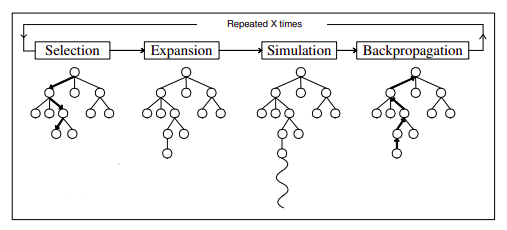
\includegraphics[width=7cm]{ressources/MCTSEtapes}
		\end{center}
	\end{block}
\end{frame}